\documentclass[11pt,a4paper]{article}
\usepackage[utf8]{inputenc}
\usepackage[T1]{fontenc}
\usepackage[english]{babel}
\usepackage{graphicx}
\usepackage{amsmath}
\usepackage{amssymb}
\usepackage{geometry}
\usepackage{hyperref}
\usepackage{listings}
\usepackage{xcolor}

\geometry{margin=2.5cm}

\title{Real-Time Signal Processing \\
\large Autotune Project Report}
\author{Your Names Here}
\date{January 2025}

\begin{document}

\maketitle

\section{Introduction}

This report presents the implementation and analysis of a real-time autotune audio effect using additive synthesis. The project was developed in C/C++ using the RtAudio API for real-time audio processing.

\section{Getting Started with RtAudio API}

\subsection{Question 2: Functionality of audioprobe and duplex}

\textbf{What do these two programs do?}

\texttt{audioprobe} scans and displays information about available audio devices (channels, sampling rates, formats, device IDs). It allows identification of system audio capabilities before configuring a stream.

\texttt{duplex} implements a real-time pass-through system that captures audio from an input device and plays it back simultaneously through an output device. It demonstrates the basic RtAudio callback structure used for real-time processing.

\subsection{Question 3a: Roles of openStream() and inout()}

\textbf{What are the roles of these two functions? Identify the arguments of openStream() and inout() for exchanging data between main and audio callback.}

\texttt{openStream()} configures and initializes the audio stream by setting device parameters, audio format (RTAUDIO\_FLOAT64), sampling rate, buffer size, callback function pointer, and user data. It prepares the audio processing pipeline before real-time execution.

\texttt{inout()} is the callback function called automatically at regular intervals to process audio in real-time. It reads samples from the input buffer, performs signal processing, and writes to the output buffer within strict timing constraints to avoid dropouts.

The key arguments for data exchange are \texttt{void *outputBuffer} (data to speakers), \texttt{void *inputBuffer} (data from microphone), and \texttt{void *userData} (user-defined structure passed from main containing buffer sizes, audio files, or dump buffers). These void pointers must be cast to their actual types within the callback.

\section{Debugging Toolbox}

\subsection{Question 4: Loading Audio Files}

\textbf{Where do you place the loading of the audio file in the program, and why?}

Audio file loading is placed in \texttt{main()} before starting the stream. File I/O operations (fopen, fread) are blocking and non-deterministic, taking unpredictable time based on disk performance. Performing them in \texttt{inout()} would cause buffer underruns and dropouts. The file only needs loading once at initialization, and memory allocation must occur before real-time processing to avoid non-deterministic behavior. By loading in main() and passing a pointer via userData, the entire file becomes available to all callbacks for sequential access.

\subsection{Question 7: Buffer Initialization}

\textbf{Do you initialize it in main() or inout() and why?}

\texttt{buffer\_dump} is initialized in \texttt{main()} before starting the stream. Dynamic memory allocation (malloc, calloc) is non-deterministic and causes delays leading to buffer underruns if performed in the callback. The buffer must persist across all callbacks to accumulate data; initializing in \texttt{inout()} would recreate it each call, losing previous data. Initialization in main() allows proper cleanup with free() at termination. A pointer is passed via userData for incremental writing during callbacks.

\subsection{Question 9: Writing to Disk}

\textbf{Do you write it in main() or inout() and why?}

\texttt{buffer\_dump} is written to disk in \texttt{main()} after stopping the stream. File operations (fopen, fwrite, fclose) are blocking and non-deterministic, taking significant time based on file size and disk performance. Performing them in \texttt{inout()} would cause severe underruns compromising real-time operation. Writing in main() ensures complete data capture in one operation rather than multiple partial writes. During callbacks, data is only copied to the buffer using \texttt{write\_buff\_dump()} (fast, deterministic), while the actual disk write occurs once at program end, separating real-time and non-real-time operations.

\section{Signal Analysis}

\subsection{Question 12: Fundamental Frequency Estimation}

\textbf{Include in your report your plots of $f_0$ as well as the files containing the corresponding input signals. Comment on your results.}

The fundamental frequency $f_0$ was estimated using the autocorrelation method. For each input buffer, the autocorrelation function was computed, and the second maximum was identified to determine the period of the signal, from which $f_0$ was calculated as:

\begin{equation}
f_0 = \frac{f_s}{\tau}
\end{equation}

where $f_s$ is the sampling rate (44100 Hz) and $\tau$ is the lag corresponding to the second maximum of the autocorrelation.

\begin{figure}[h]
    \centering
    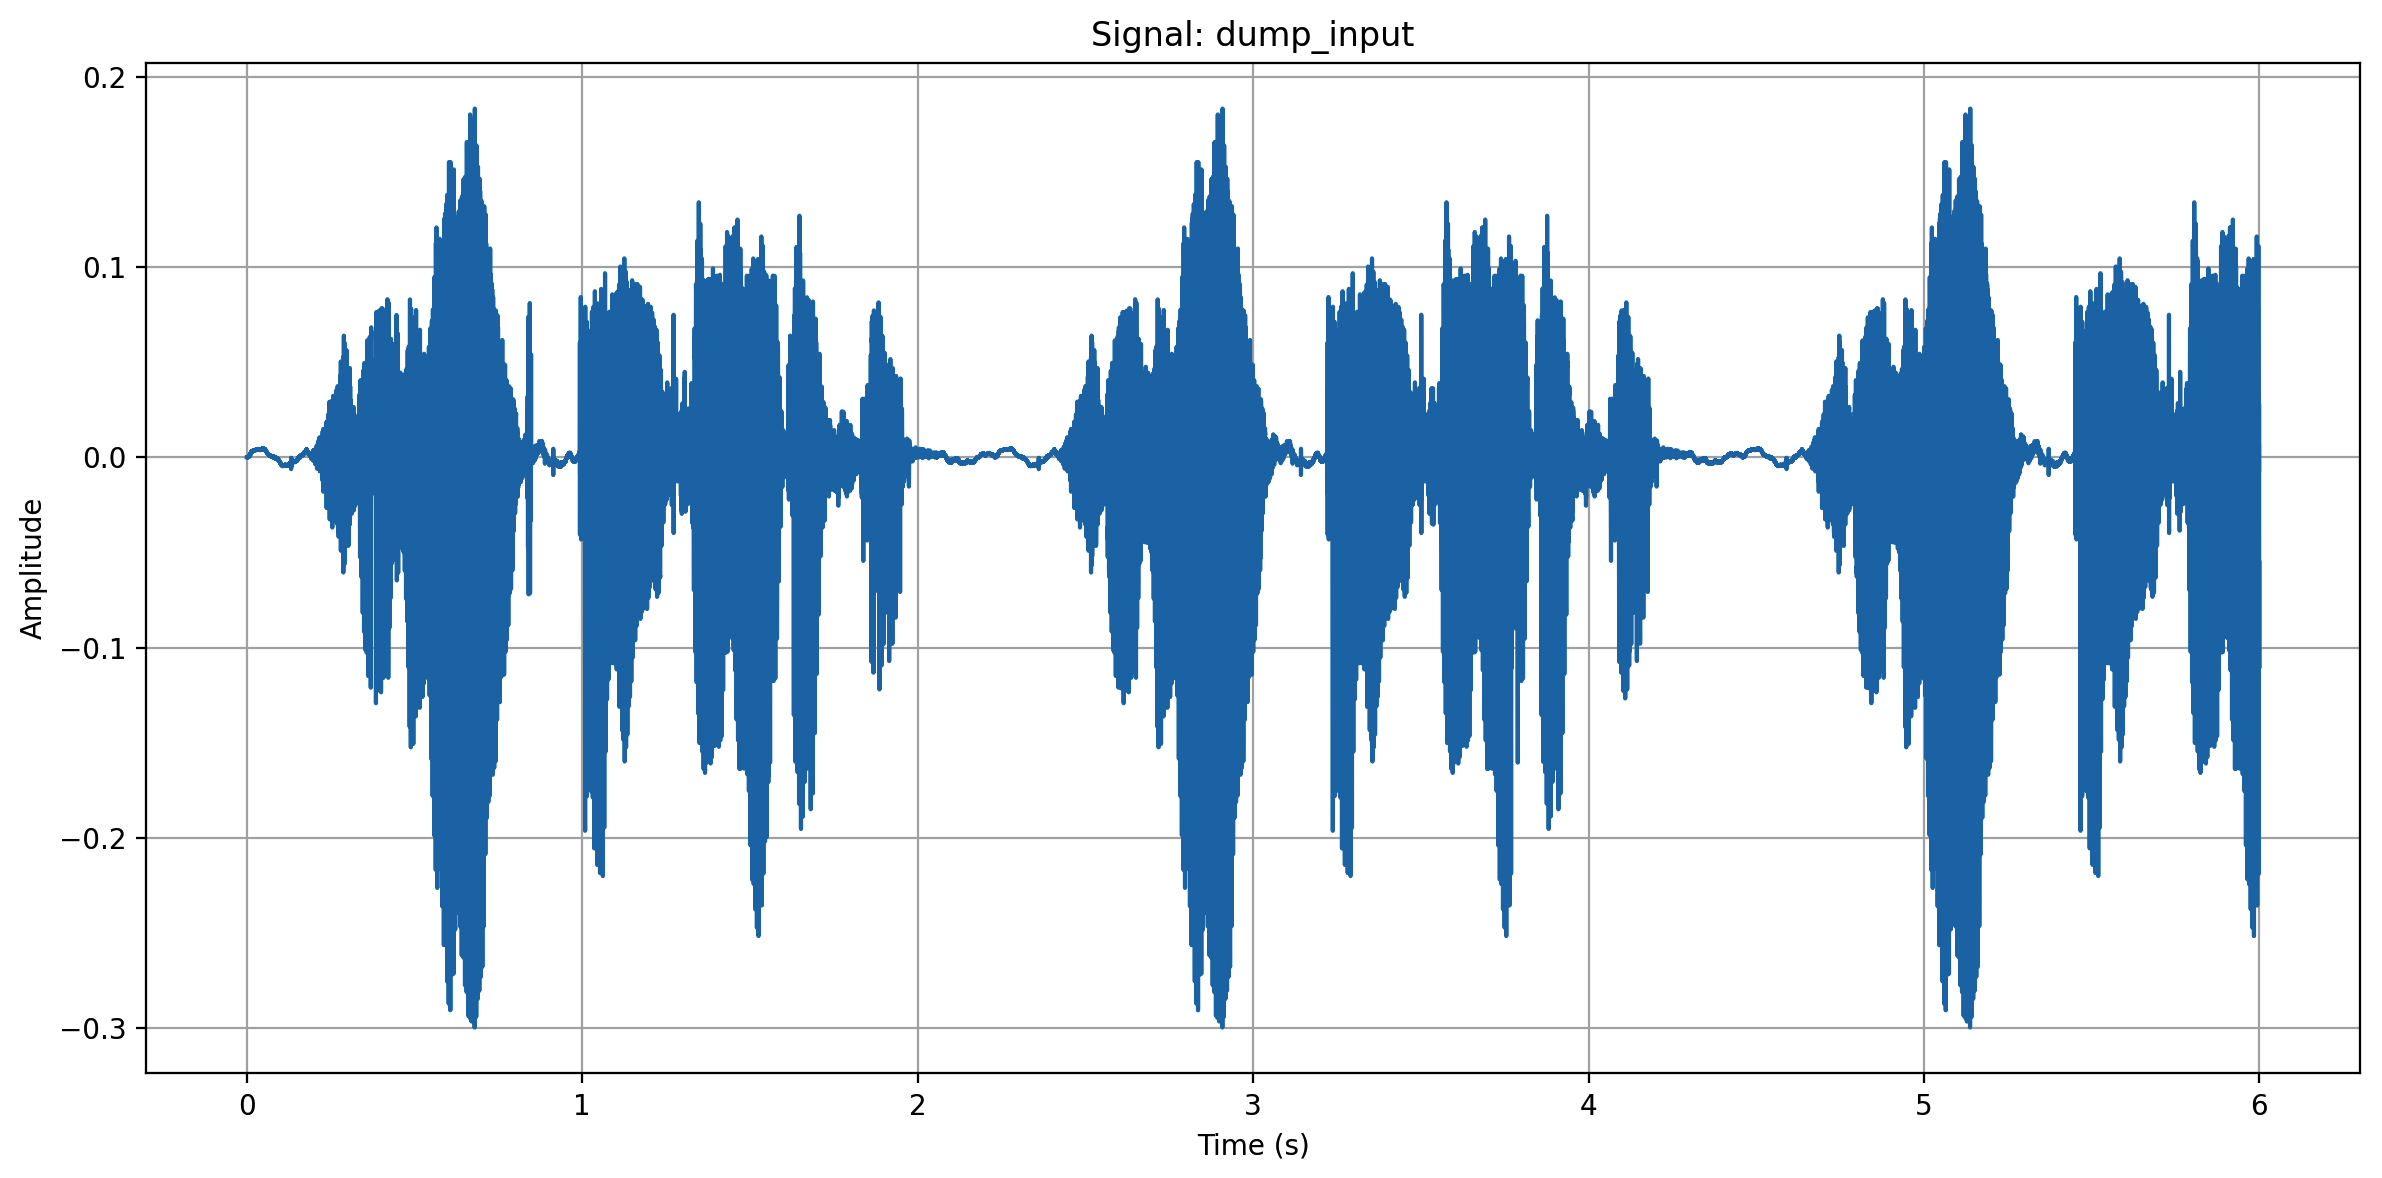
\includegraphics[width=0.8\textwidth]{F01_a3_s100_v04.png}
    \caption{Input signal F01\_a3\_s100\_v04 (female voice)}
    \label{fig:input_signal}
\end{figure}

\begin{figure}[h]
    \centering
    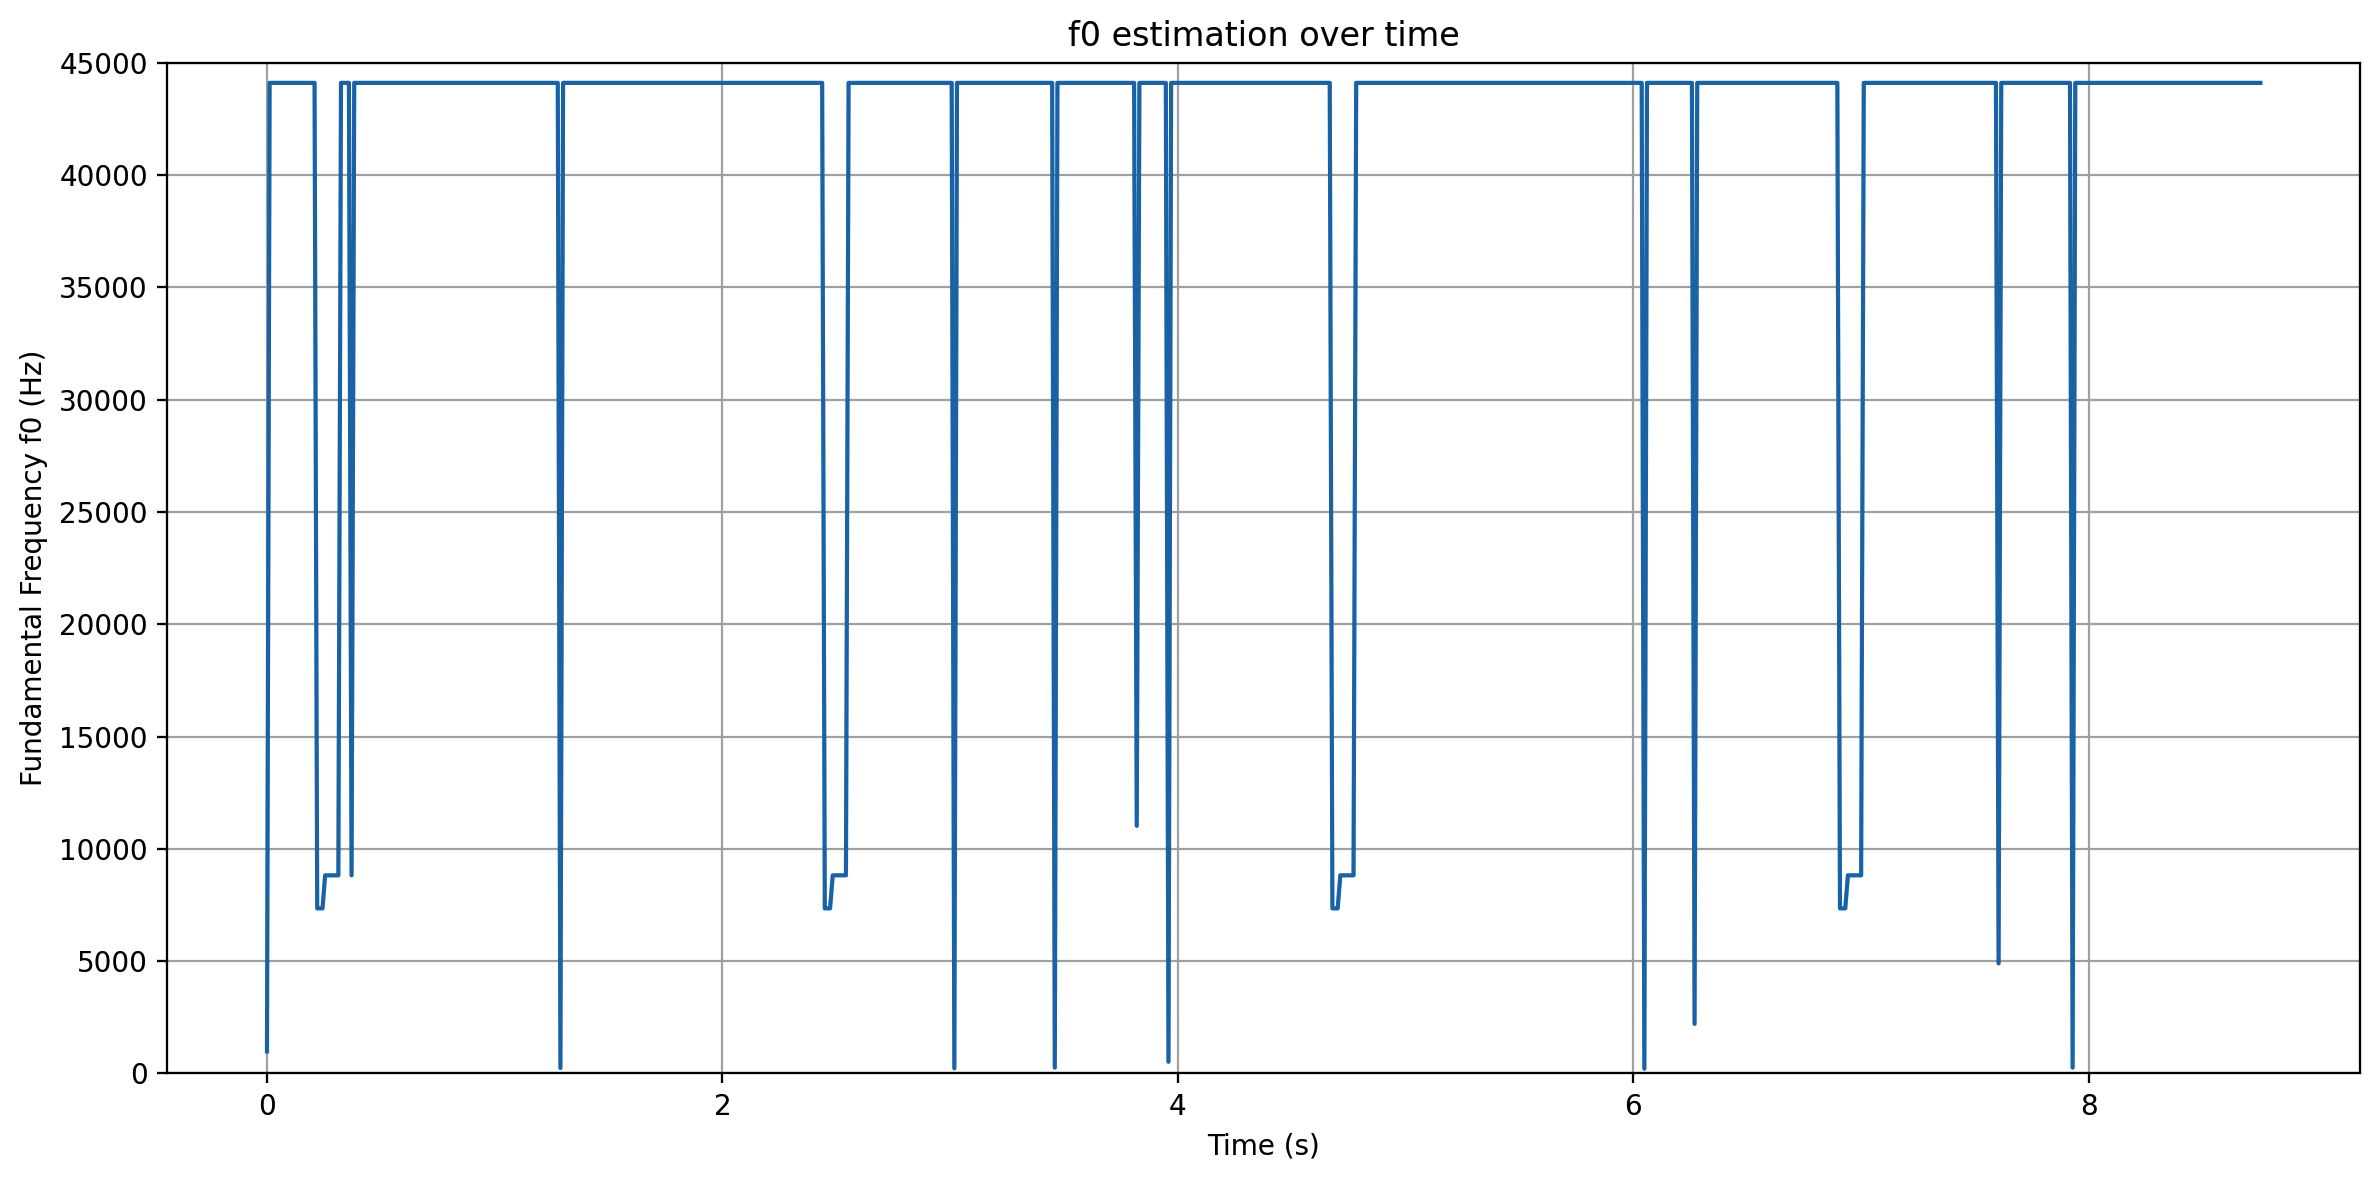
\includegraphics[width=0.8\textwidth]{f0-without_frequency_range-512.png}
    \caption{$f_0$ estimation without frequency range limitation (buffer size 512)}
    \label{fig:f0_no_limit}
\end{figure}

\begin{figure}[h]
    \centering
    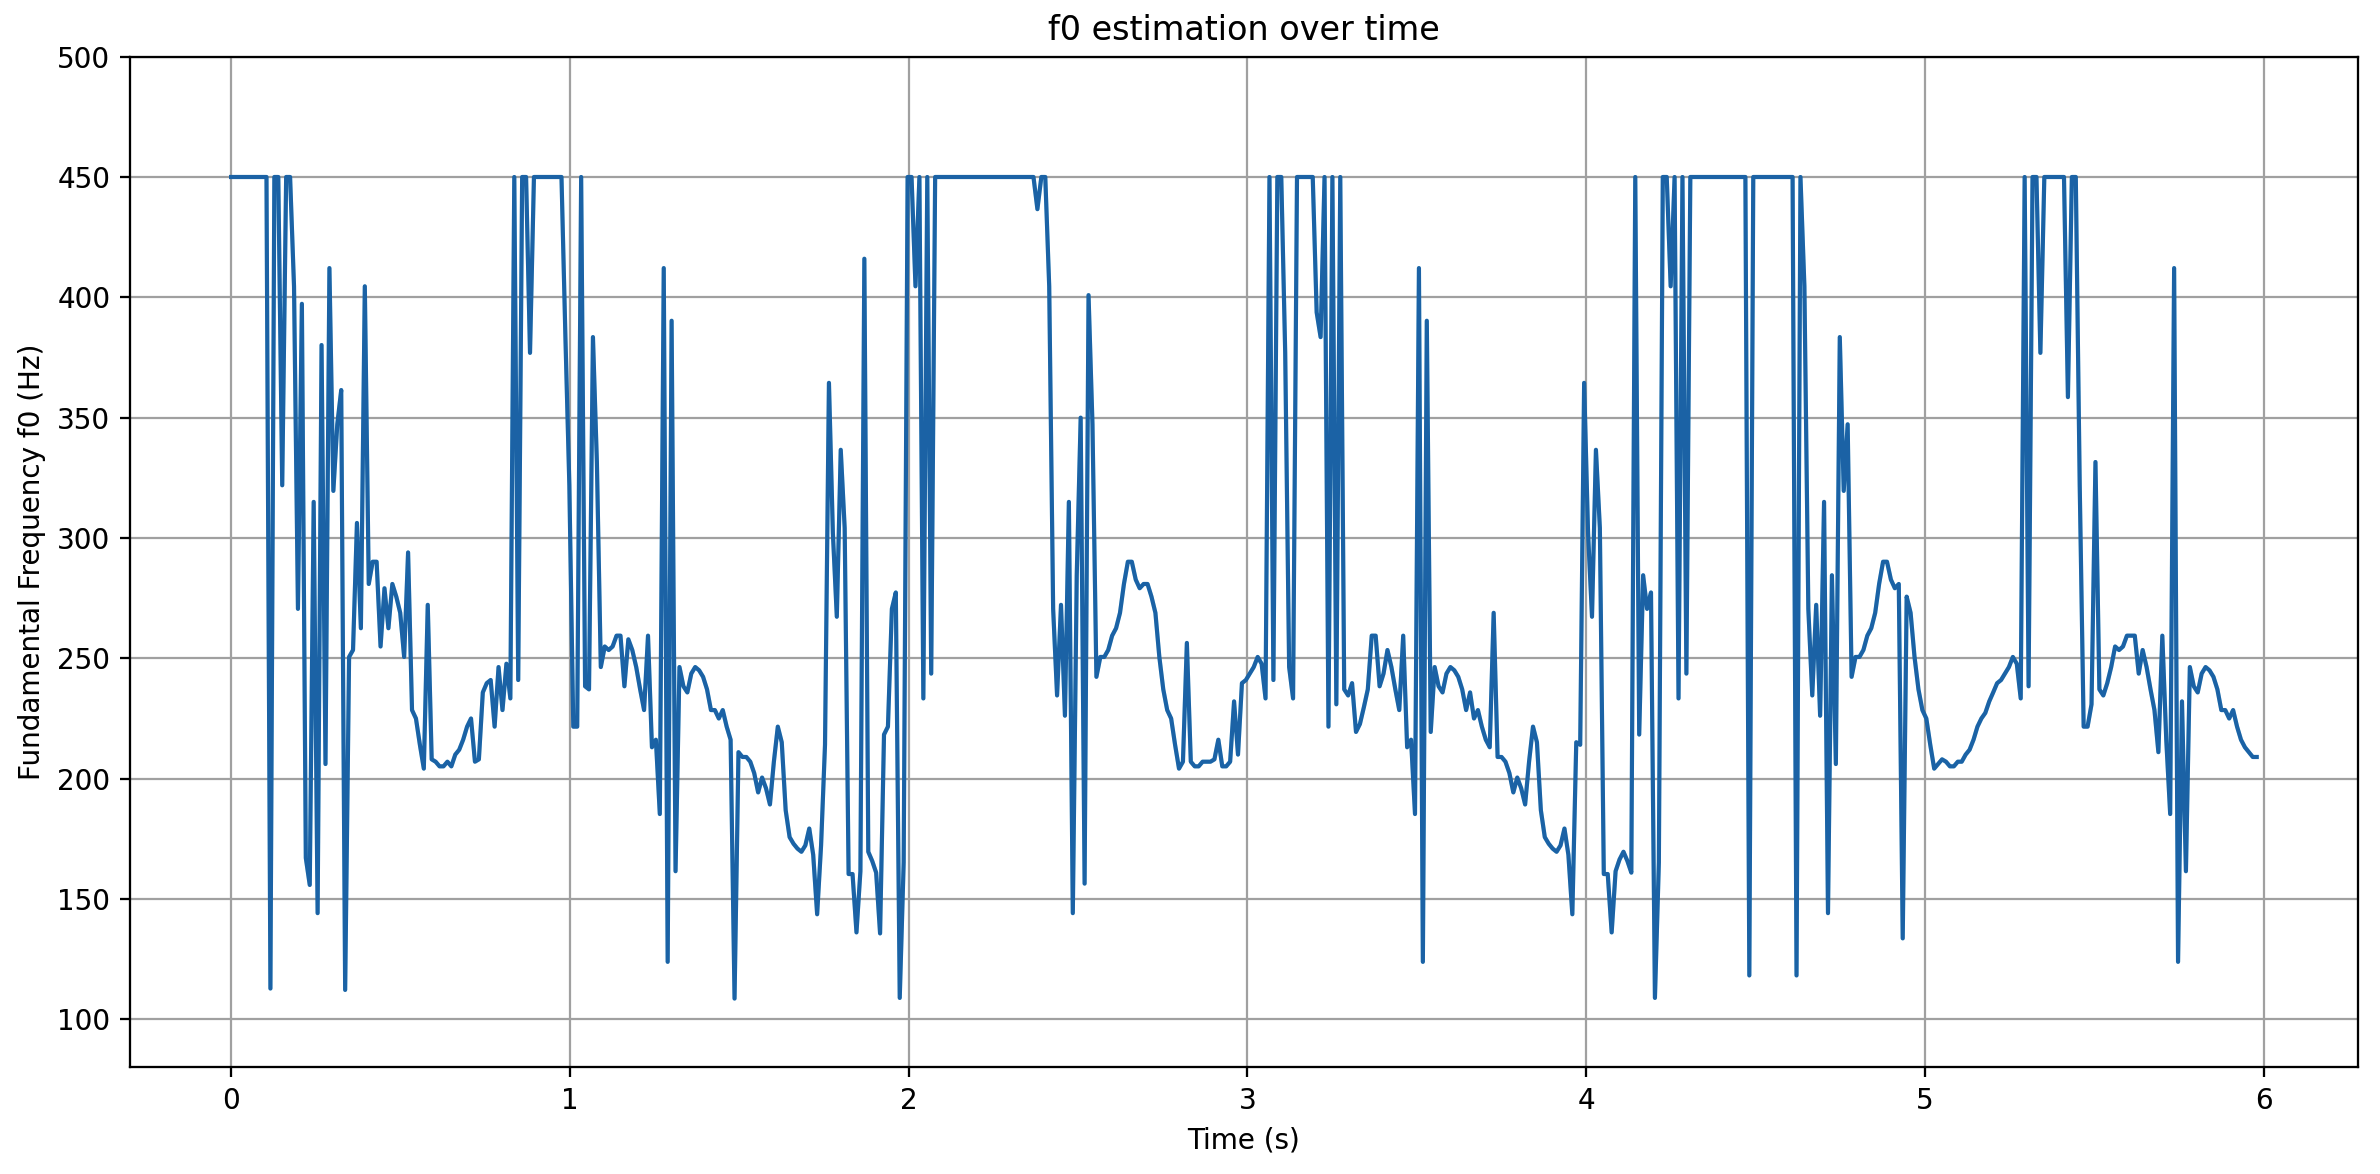
\includegraphics[width=0.8\textwidth]{f0-512.png}
    \caption{$f_0$ estimation with frequency range limitation 80-450 Hz (buffer size 512)}
    \label{fig:f0_limited}
\end{figure}

\textbf{Analysis and comments:}

The input signal F01\_a3\_s100\_v04 (Figure \ref{fig:input_signal}) is a sustained vowel from a female speaker with clear periodic structure during voiced segments and lower amplitude during silent periods.

Without frequency range limitation (Figure \ref{fig:f0_no_limit}), the autocorrelation method produces highly erratic $f_0$ estimates with values exceeding 1000 Hz and frequent jumps. This demonstrates the critical importance of constraining the search range. Unvoiced segments and low-amplitude regions trigger false detections at arbitrary lags, producing unrealistic frequency values.

With frequency range limitation to 80-450 Hz (Figure \ref{fig:f0_limited}), the $f_0$ estimation is dramatically improved. The trajectory shows a stable fundamental frequency around 200-250 Hz during voiced segments, consistent with typical female vocal range. The temporal evolution reveals natural pitch variations corresponding to prosodic patterns. However, some octave errors ($f_0/2$) are still visible as occasional drops to approximately 100-125 Hz, particularly during segment transitions or low-energy frames. These errors occur when the autocorrelation's second maximum corresponds to twice the actual period rather than the fundamental period.

\subsection{Question 14: Buffer Size Analysis and Circular Buffer}

\textbf{Provide the corresponding plots and comment. Why would a circular buffer be useful here?}

\begin{figure}[h]
    \centering
    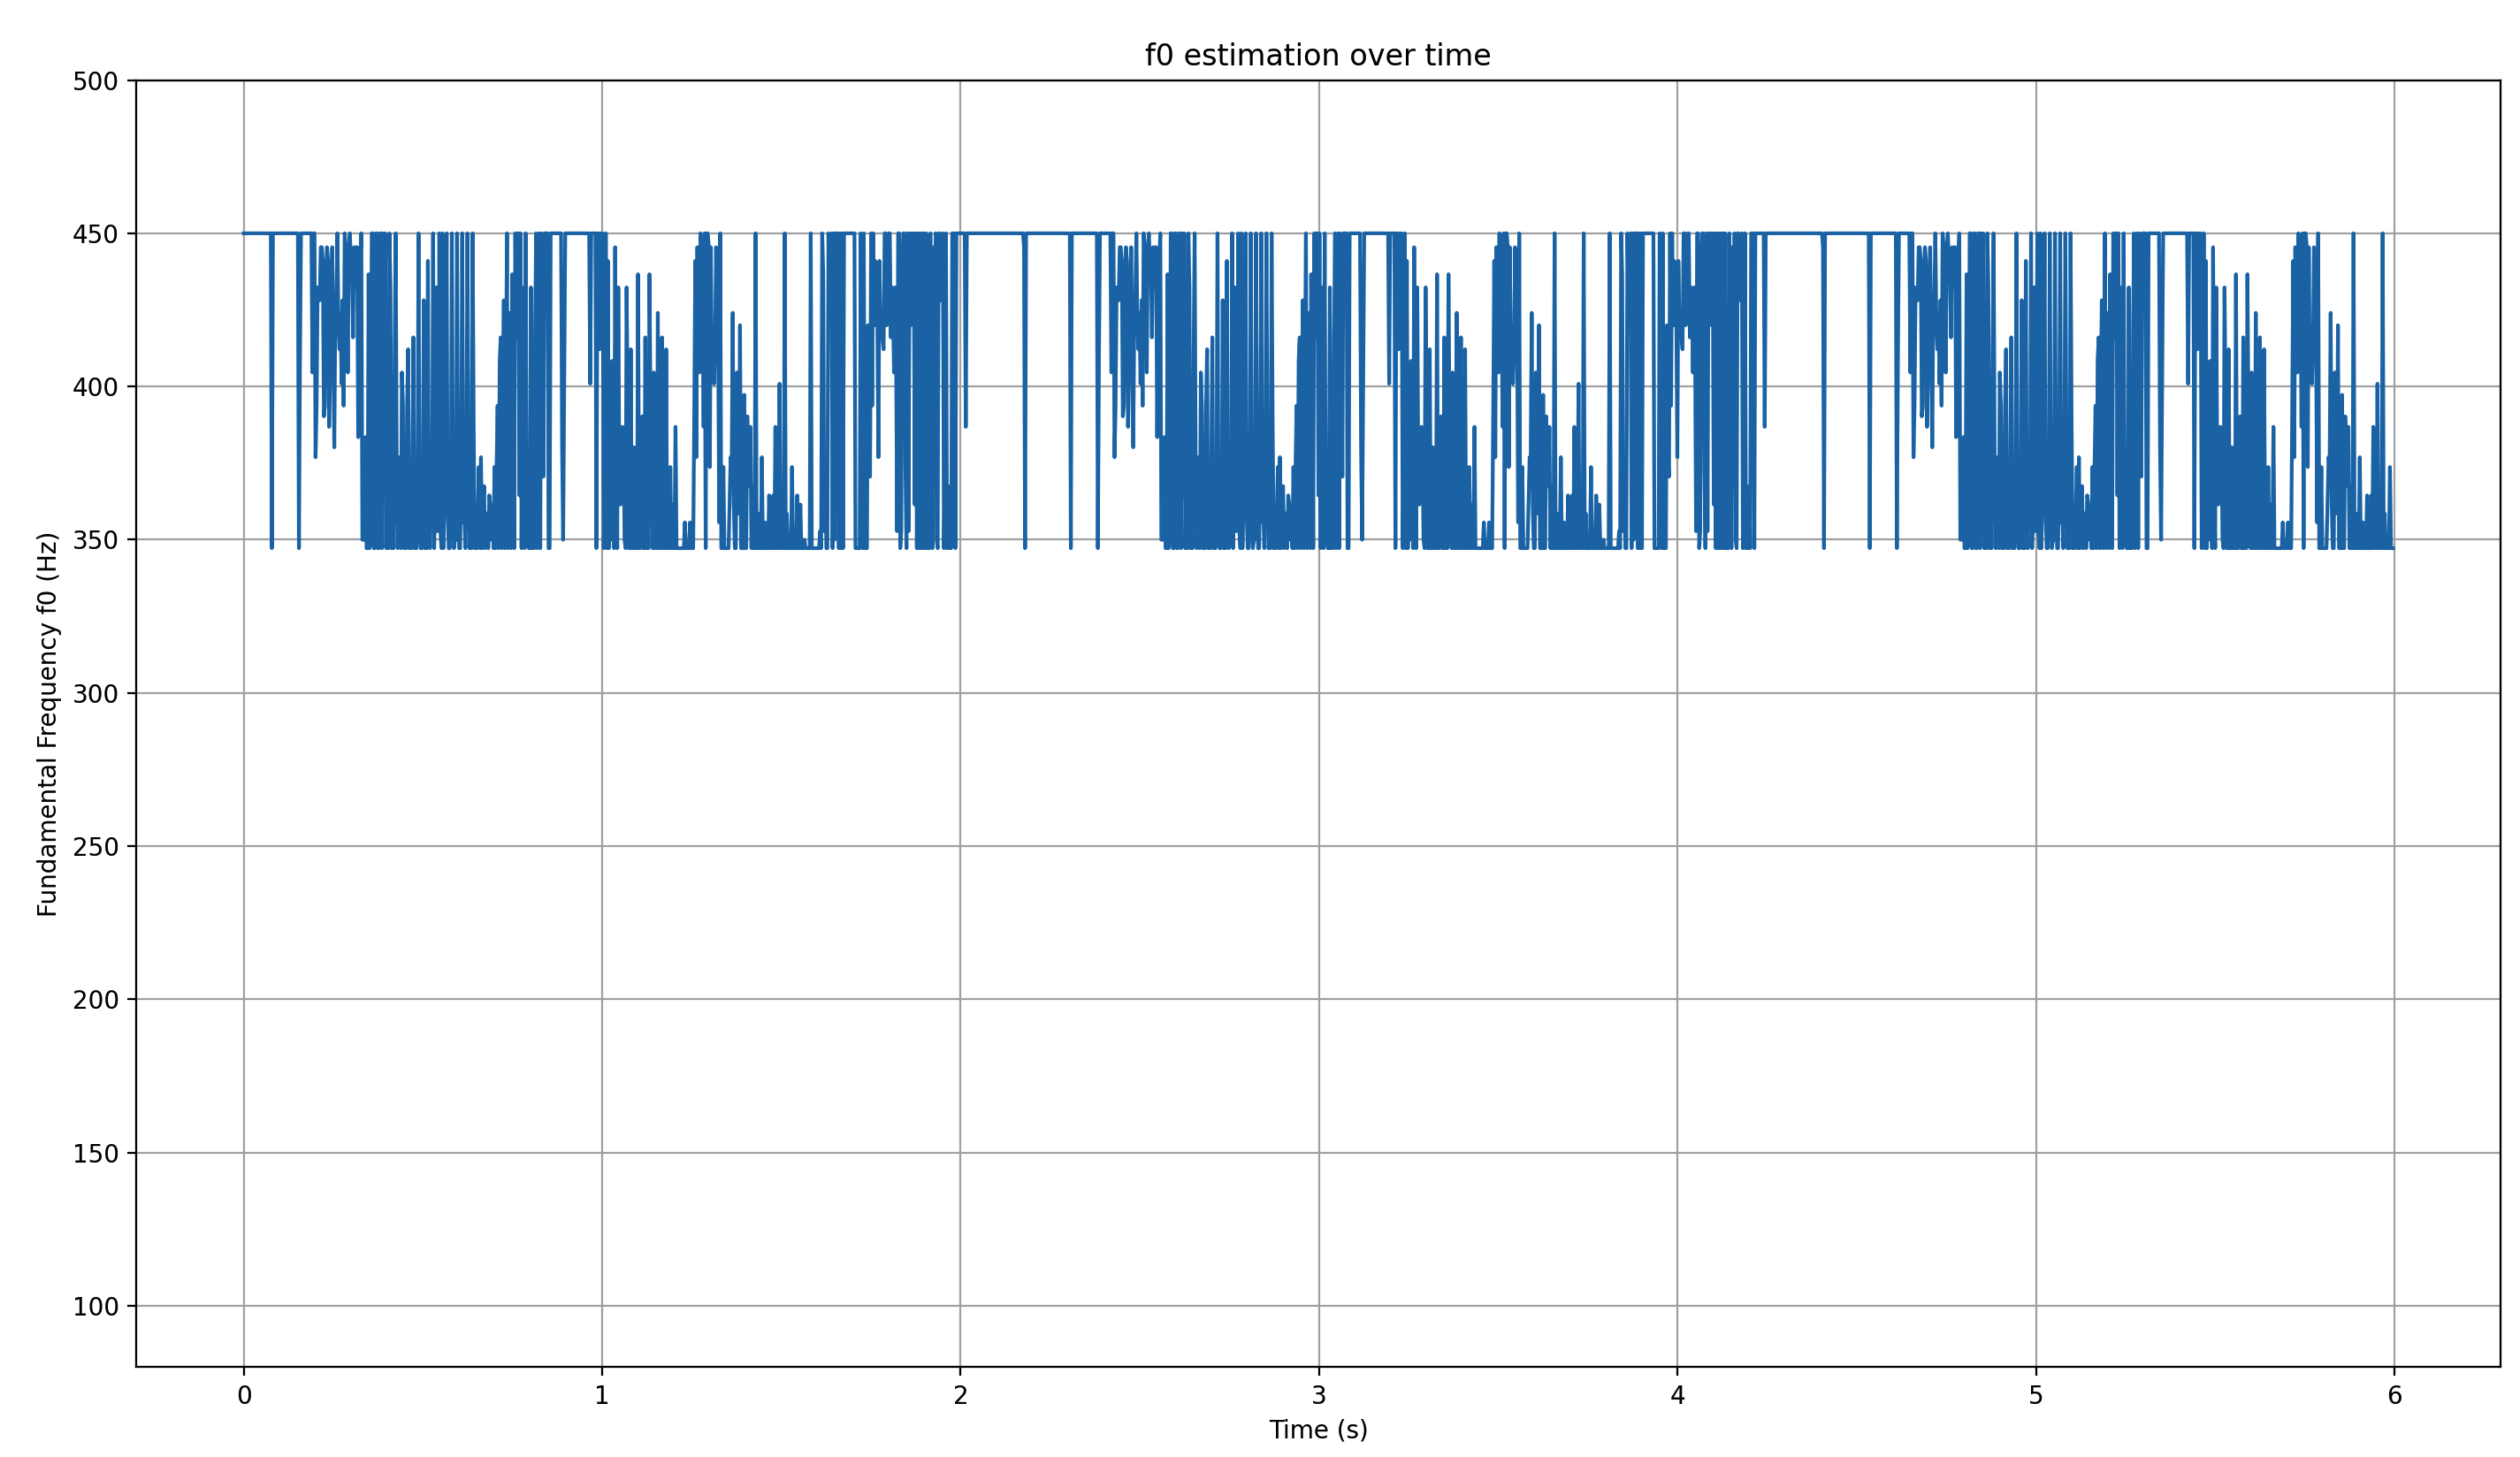
\includegraphics[width=0.7\textwidth]{f0-128.png}
    \caption{$f_0$ estimation with buffer size N=128}
    \label{fig:f0_128}
\end{figure}

\begin{figure}[h]
    \centering
    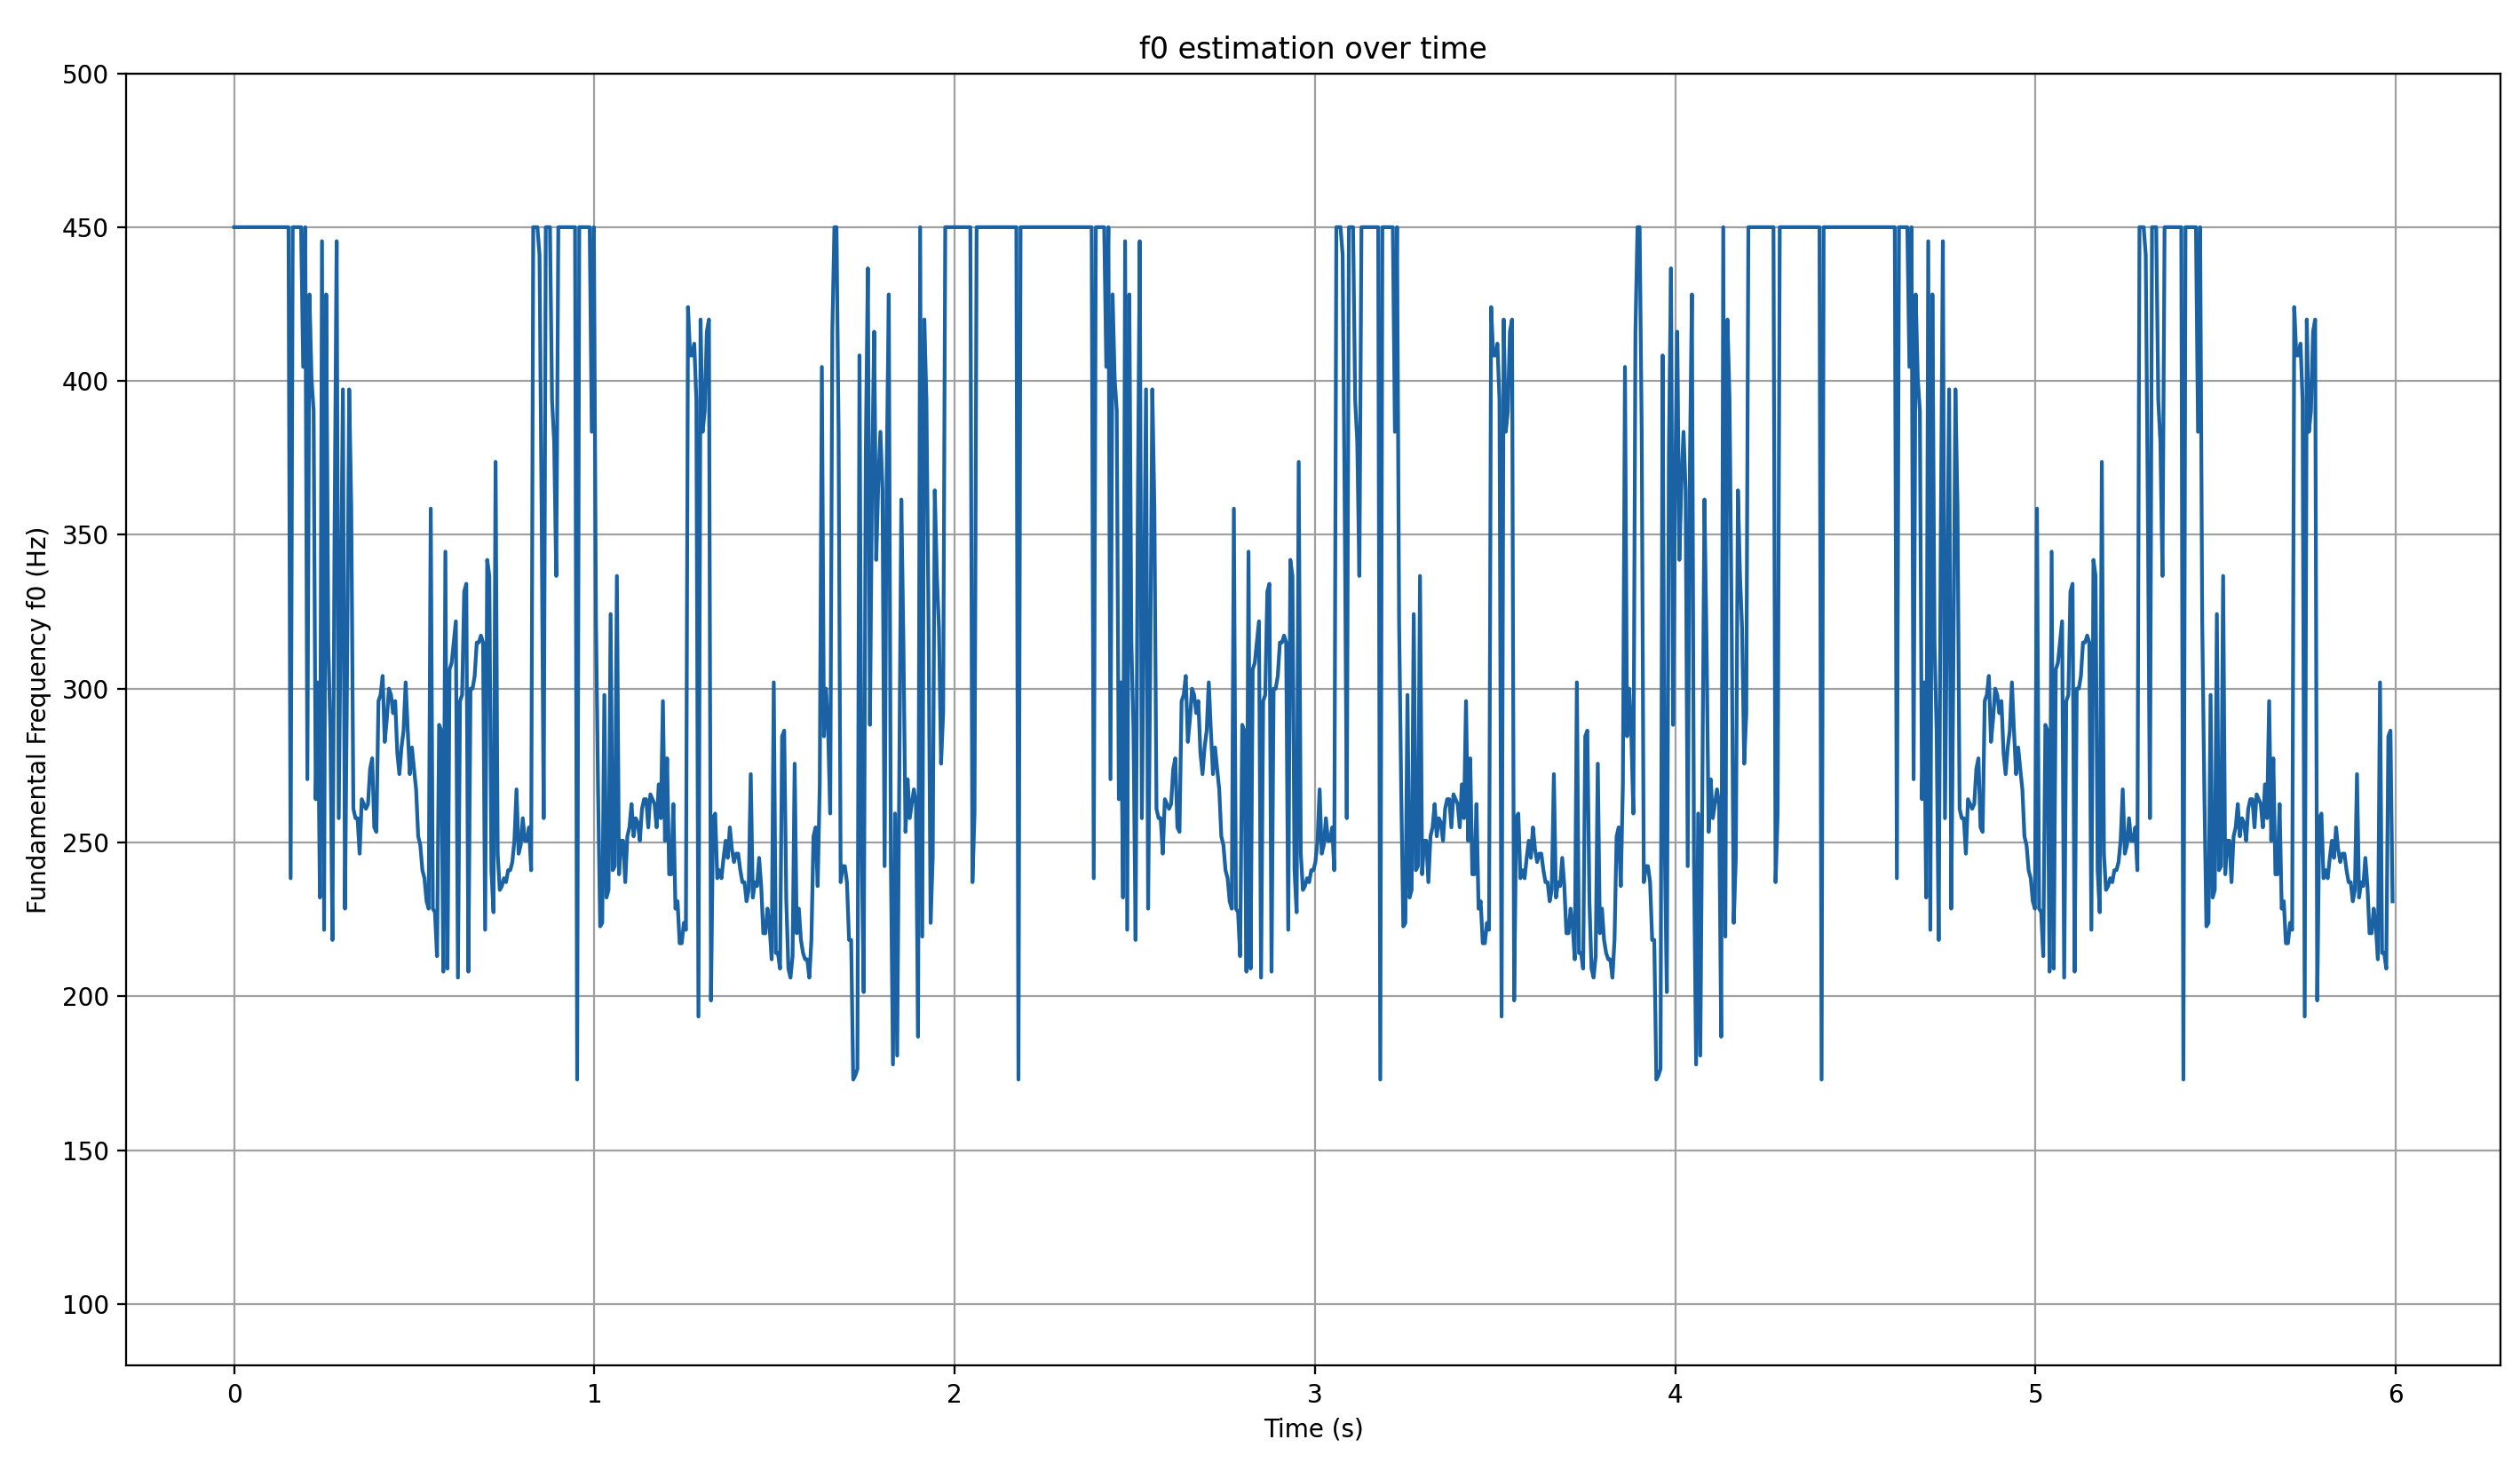
\includegraphics[width=0.7\textwidth]{f0-256.png}
    \caption{$f_0$ estimation with buffer size N=256}
    \label{fig:f0_256}
\end{figure}

\begin{figure}[h]
    \centering
    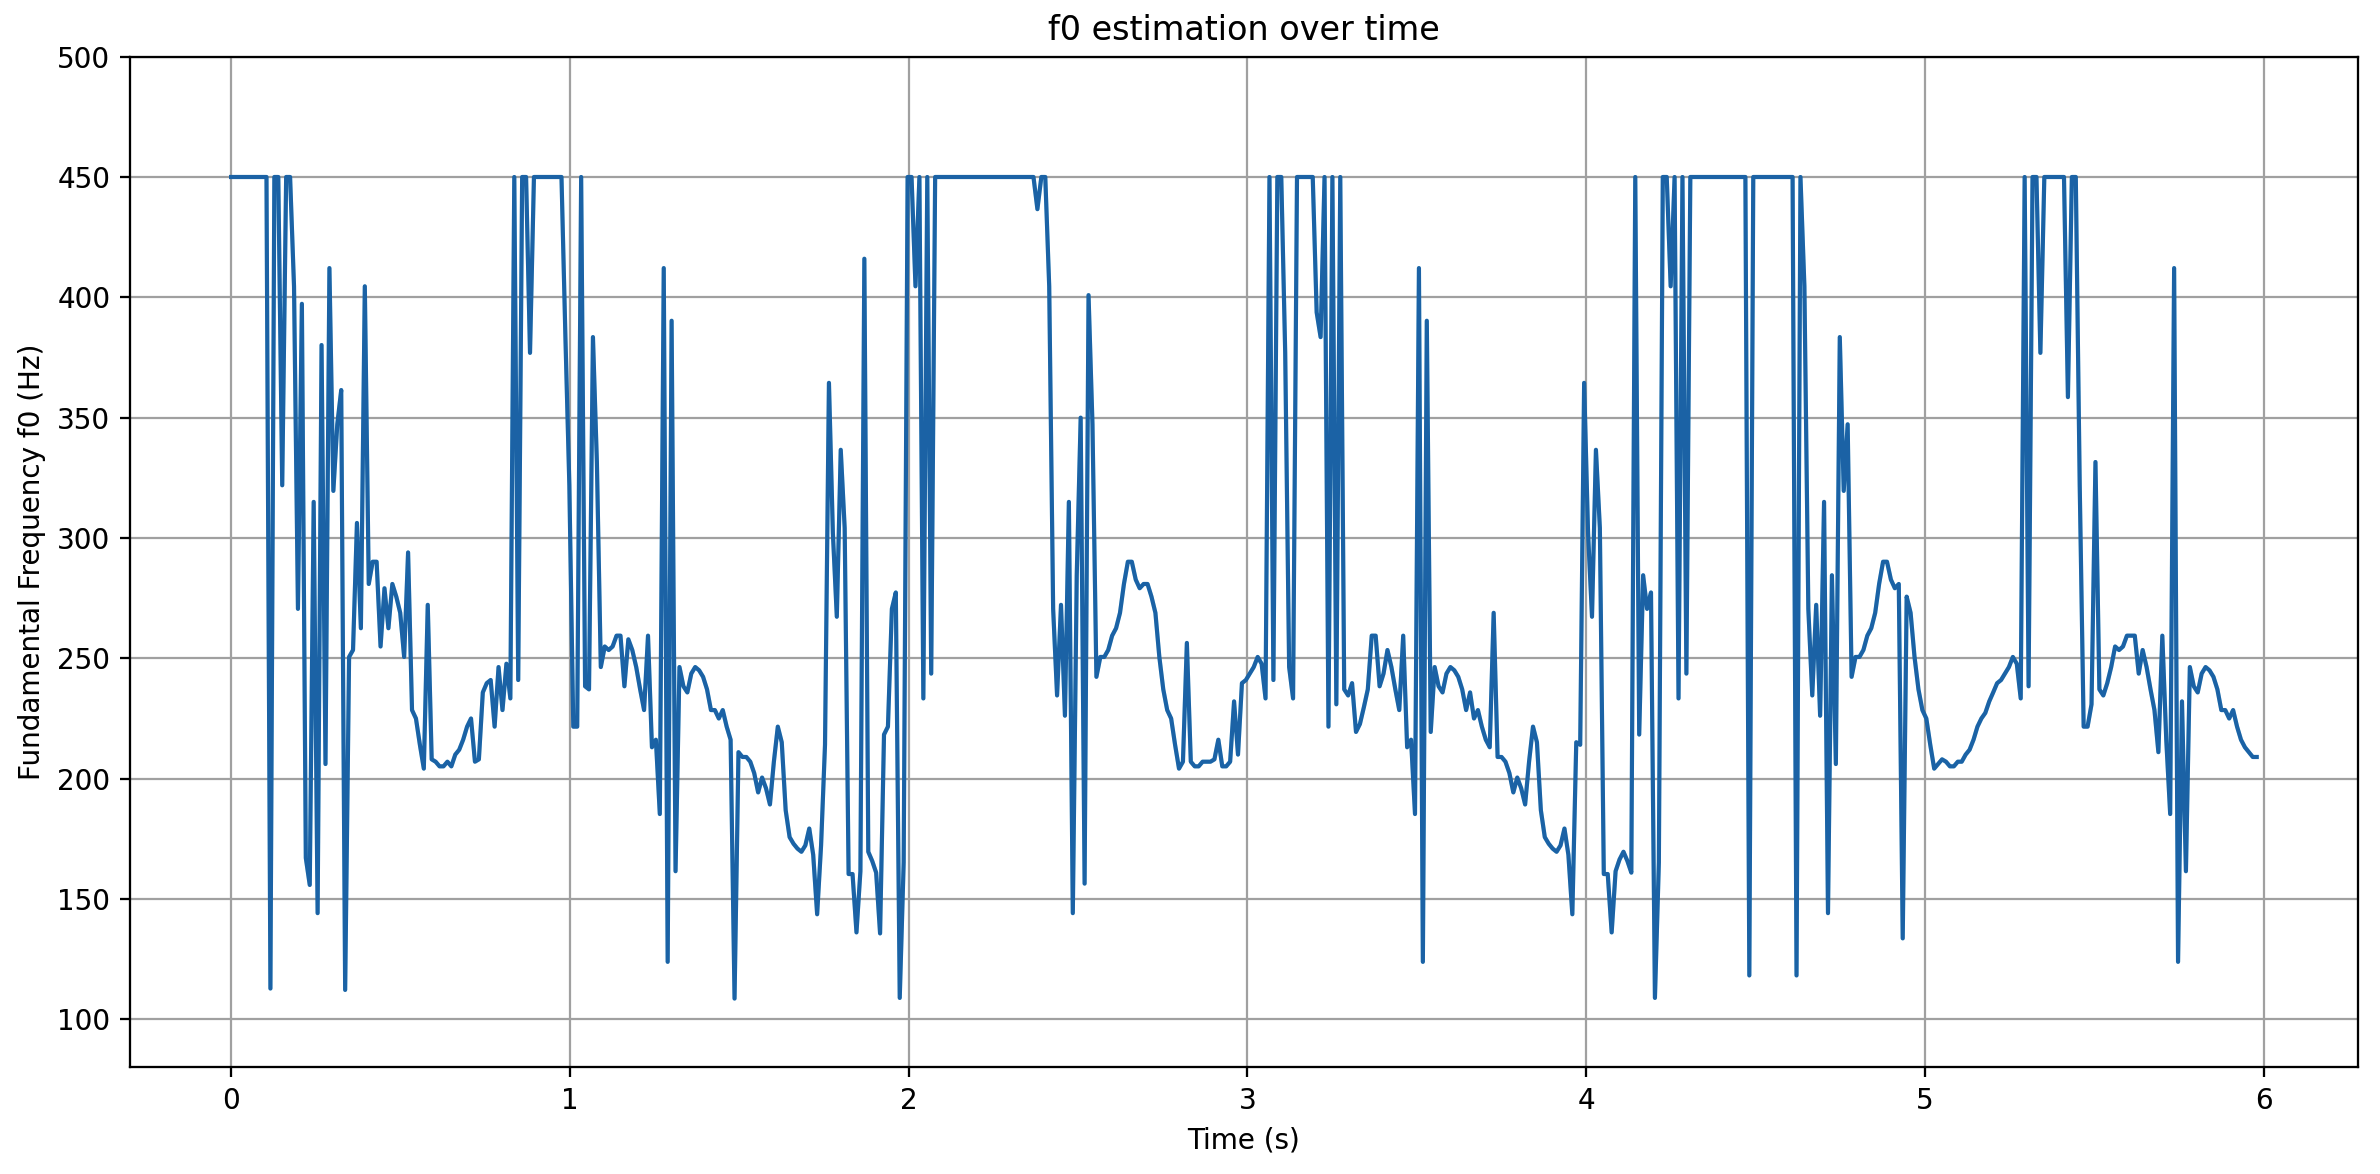
\includegraphics[width=0.7\textwidth]{f0-512.png}
    \caption{$f_0$ estimation with buffer size N=512}
    \label{fig:f0_512}
\end{figure}

\begin{figure}[h]
    \centering
    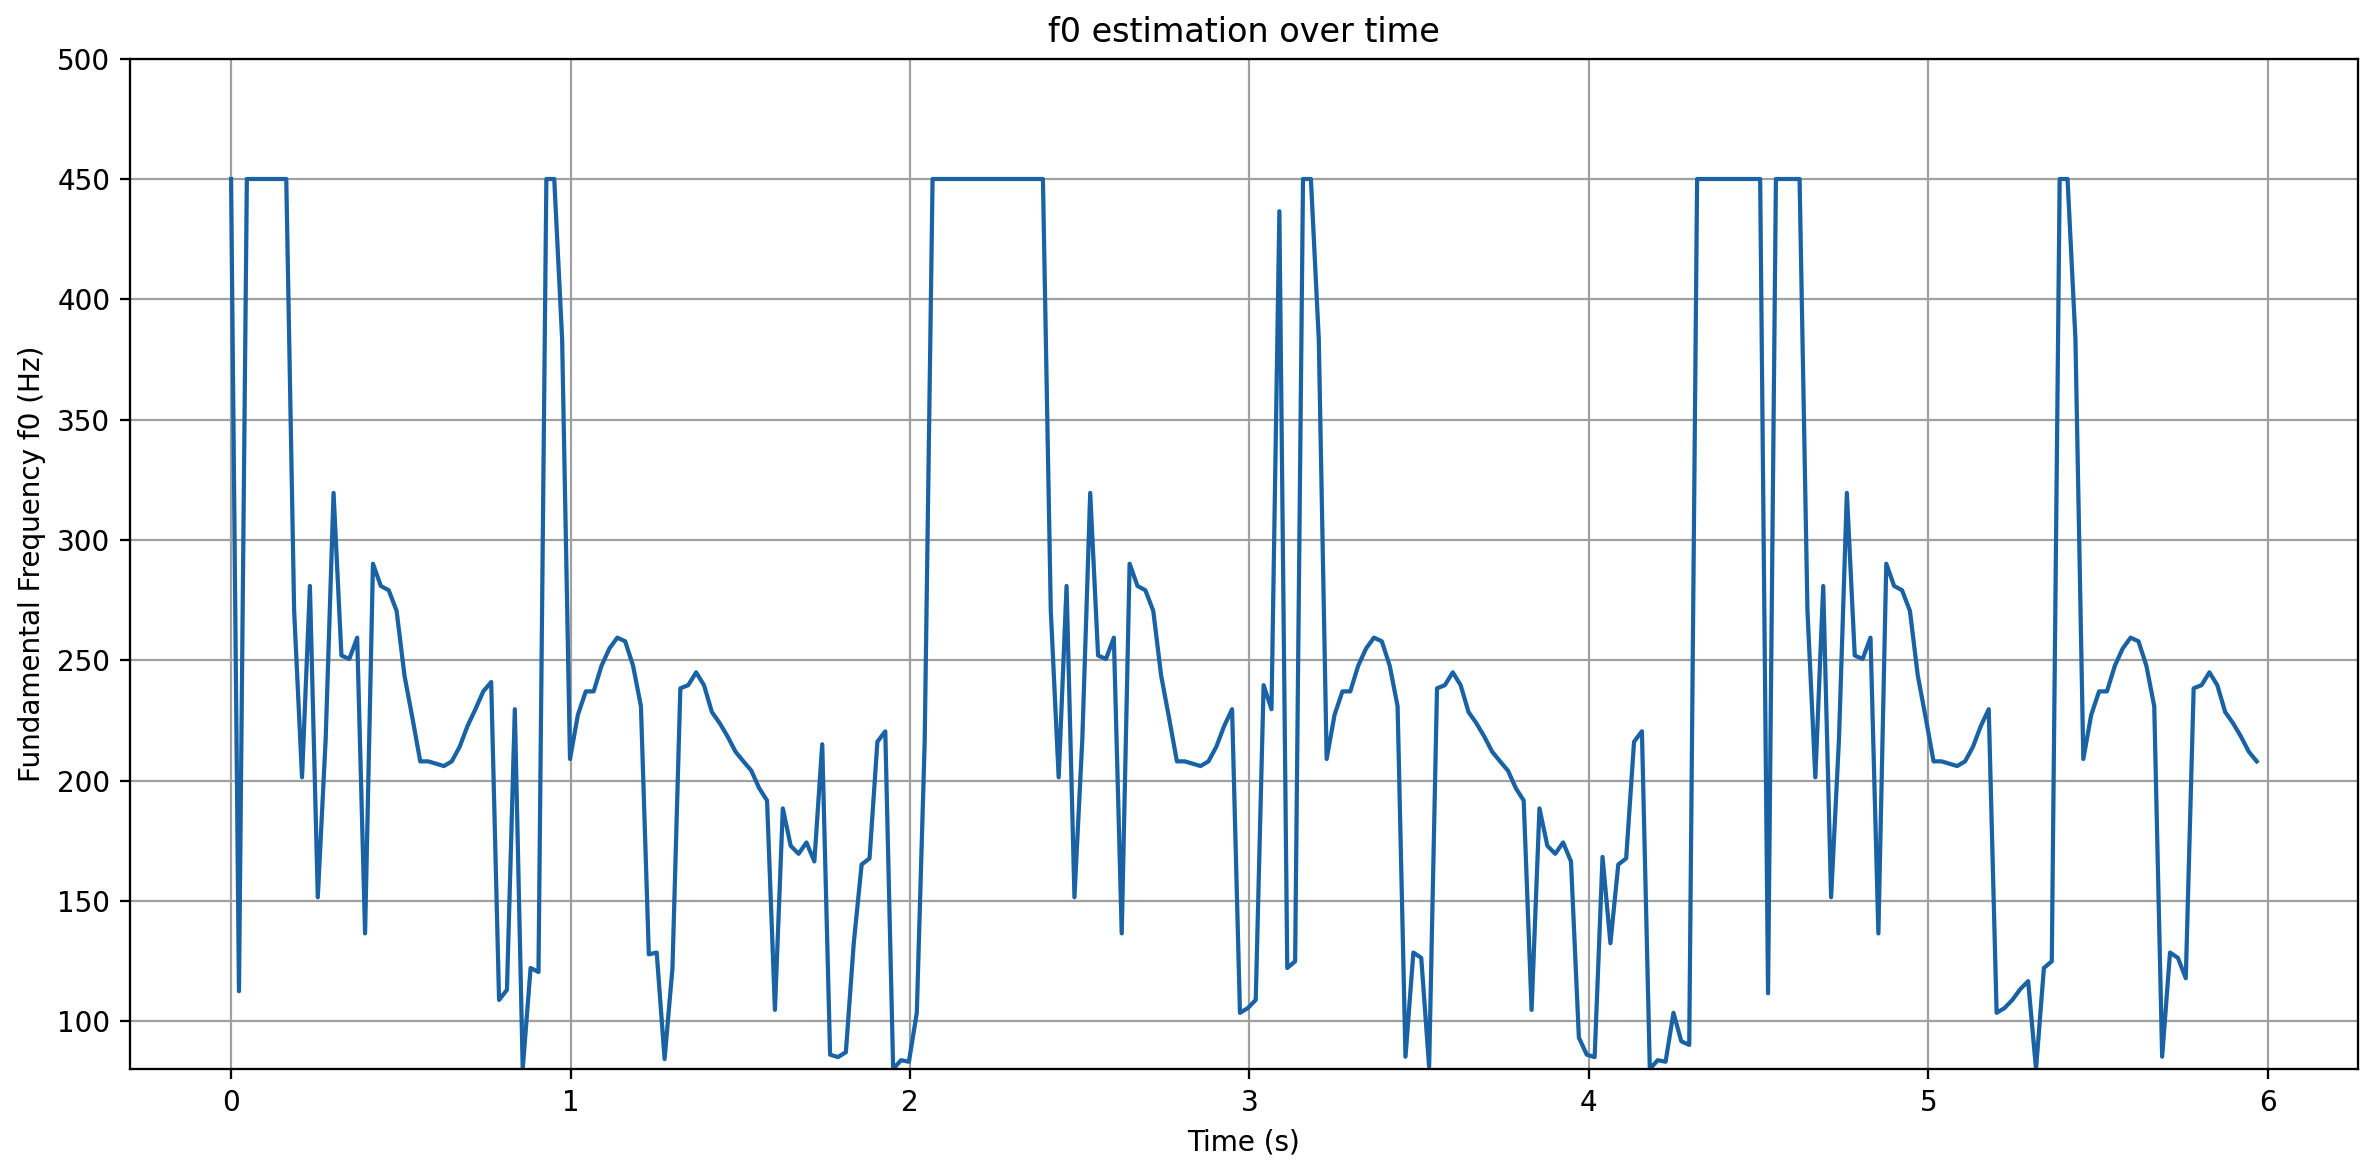
\includegraphics[width=0.7\textwidth]{f0-1024.png}
    \caption{$f_0$ estimation with buffer size N=1024}
    \label{fig:f0_1024}
\end{figure}

\begin{figure}[h]
    \centering
    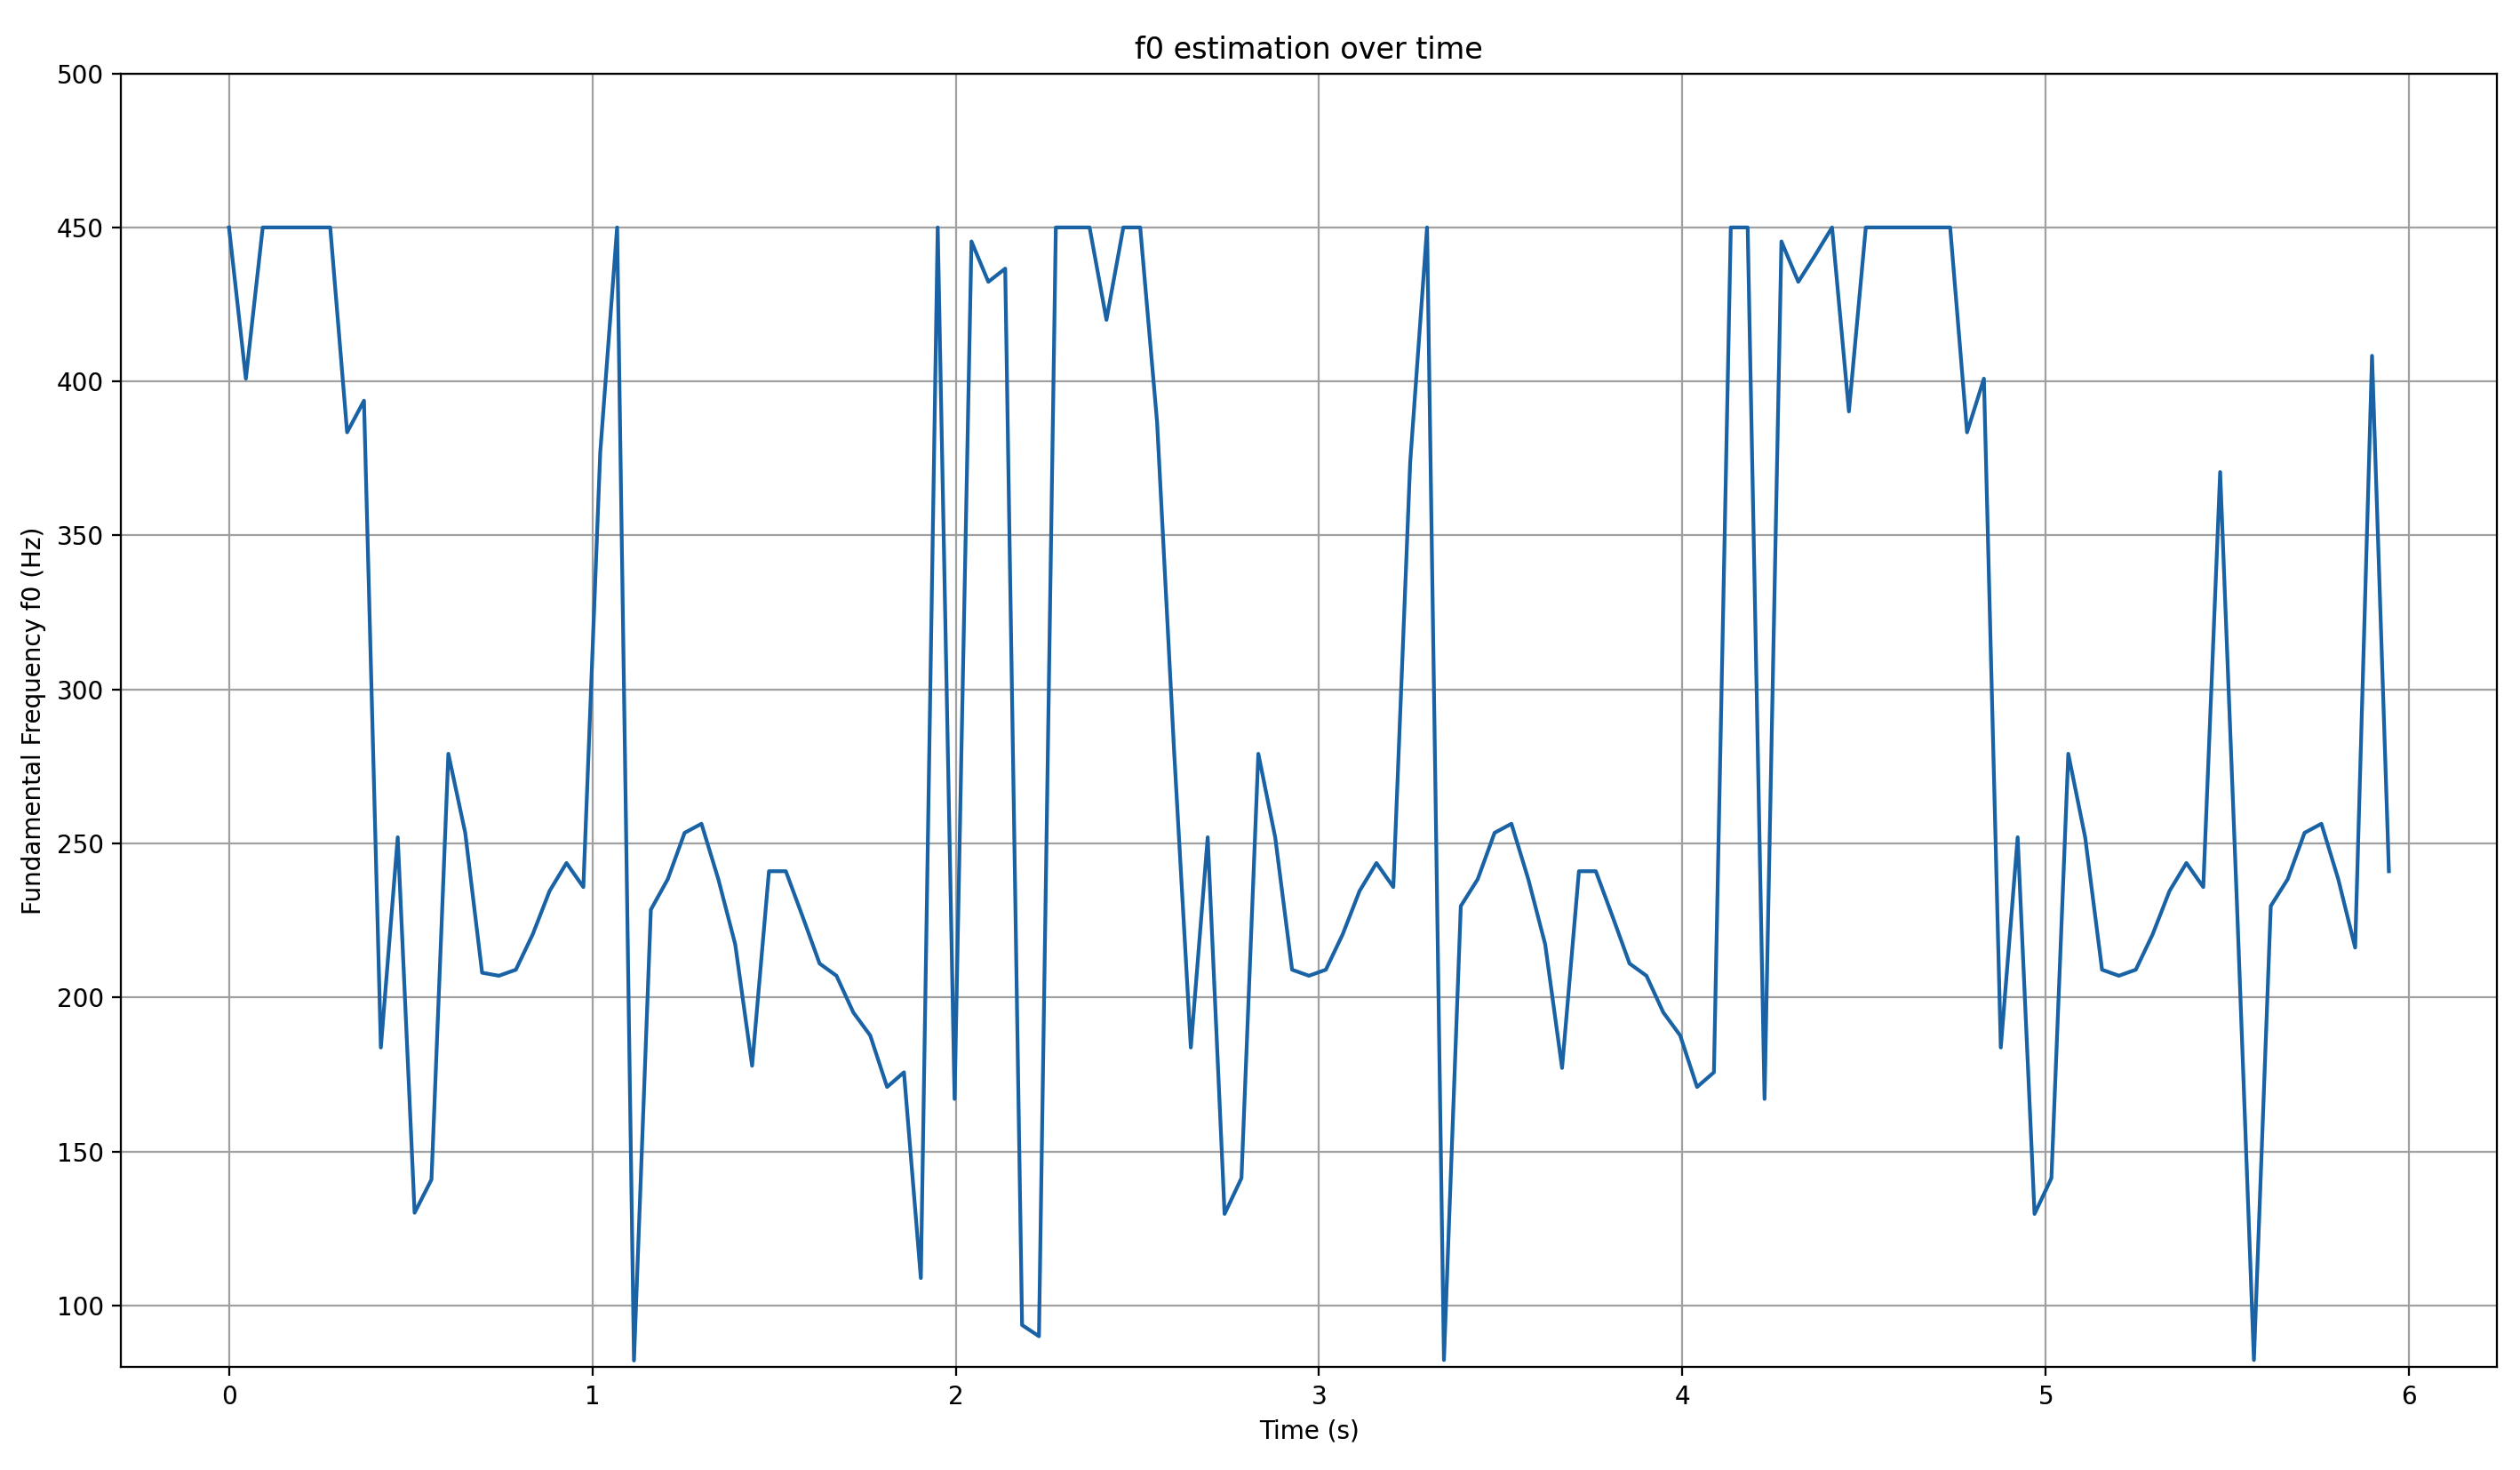
\includegraphics[width=0.7\textwidth]{f0-2048.png}
    \caption{$f_0$ estimation with buffer size N=2048}
    \label{fig:f0_2048}
\end{figure}

\textbf{Analysis of buffer size effects:}

The comparison of buffer sizes from 128 to 2048 samples reveals clear trade-offs. With N=128 (Figure \ref{fig:f0_128}), the $f_0$ trajectory is extremely noisy with frequent octave errors and spurious values, as the short analysis window cannot reliably capture complete pitch periods for the ~200 Hz fundamental (requiring ~220 samples at 44100 Hz). The estimation is unstable throughout.

At N=256 (Figure \ref{fig:f0_256}), performance improves slightly but remains highly erratic with persistent octave jumps and detection failures. At N=512 (Figure \ref{fig:f0_512}), the trajectory becomes more stable with reduced jitter, though octave errors still occur occasionally during transitions.

With N=1024 (Figure \ref{fig:f0_1024}), the estimation quality significantly improves. The $f_0$ curve is smoother with fewer octave errors and more consistent tracking during voiced segments. The longer analysis window provides better frequency resolution, reducing ambiguity in peak detection.

At N=2048 (Figure \ref{fig:f0_2048}), the trajectory is the smoothest and most stable, with minimal noise and very few octave errors. However, the temporal resolution is reduced, with fewer $f_0$ estimates per second (approximately 21 Hz update rate at 44100 Hz sampling), making it slower to respond to rapid pitch changes. The increased latency (~46 ms) would be problematic for interactive real-time applications.

\textbf{Why a circular buffer is useful:}

A circular buffer decouples analysis and I/O buffer sizes, allowing $f_0$ analysis on large windows (e.g., 1024 samples) while maintaining small I/O buffers (e.g., 256 samples). This provides both low latency and high-quality estimation without compromise.

Each callback adds new samples while automatically overwriting old ones, creating a sliding window containing the most recent N samples without explicit shifting. Analyzing overlapping windows produces smoother $f_0$ trajectories with better temporal tracking than non-overlapping chunks.

Implementation requires only fixed memory allocation regardless of duration, avoiding growth issues. Using pointer arithmetic for read/write positions minimizes data movement, making it efficient for real-time processing.

\section{Conclusion}

This project implements a real-time autotune effect using additive synthesis. Key challenges addressed include separating non-real-time operations (file I/O, memory allocation) from the audio callback, implementing $f_0$ estimation via autocorrelation, balancing buffer size trade-offs between latency and accuracy, and using circular buffers for efficient sliding window analysis.

The final implementation processes audio in real-time, detecting pitch and applying autotune correction to quantize frequencies to the musical scale, demonstrating the critical importance of distinguishing real-time from non-real-time operations to meet strict timing deadlines.

\end{document}
